\chapter{Contribution} \label{chap:conclusion}

In tune with the aims and goals summarized in the previous chapter,
we consider two rather naive models, one for image classification, and one for
pointclouds. The two models however share many similarities and are in no way
tied to these particular tasks, and we only choose classification as a
playground to evaluate the models.

\section{Hyperbolic convolutions} \label{sec:hconv-new}

Developing upon a collaborative project described
in~\autoref{sec:hconv}, we propose a next
iteration of the model. Recall that in the model we construct hyperbolic
embeddings for each input image's pixel, producing a ``\( 2 \)-dimensional
array of manifold-points''. This array is then scanned with a sliding window,
and points within each window are ``aggregated'' to produce a point for the
output array. Aggregation amounts to application of some sort of ``reusable
filters'' that are deemed to match various ``patterns''. The intuition for this convolution
of ``hyperbolic arrays'' is to treat the embeddings as nodes in a ``continuous'' tree
and construct a decision rule for sinking down the tree based on ``neighbour nodes''.
We note that in the original model, the aggregation step is a function of the
``absolute positions'' of the points, measured with respect to a fixed origin.
We also note that the success of the classical (Euclidean) convolution in
``pattern-matching'' is understood to be due to its invariance properties,
specifically the invariance with respect to translations. Developing this intuition,
we propose to simply replace the \( \log_0 \) in the aggregation step
with logarithmic map \( \log_x \) from some point \( x \) in the window, thus
producing a decision rule based only on ``relative directions'' towards neighbours
and independent of ``which subtree we're in''

\begin{figure}[ht]\center
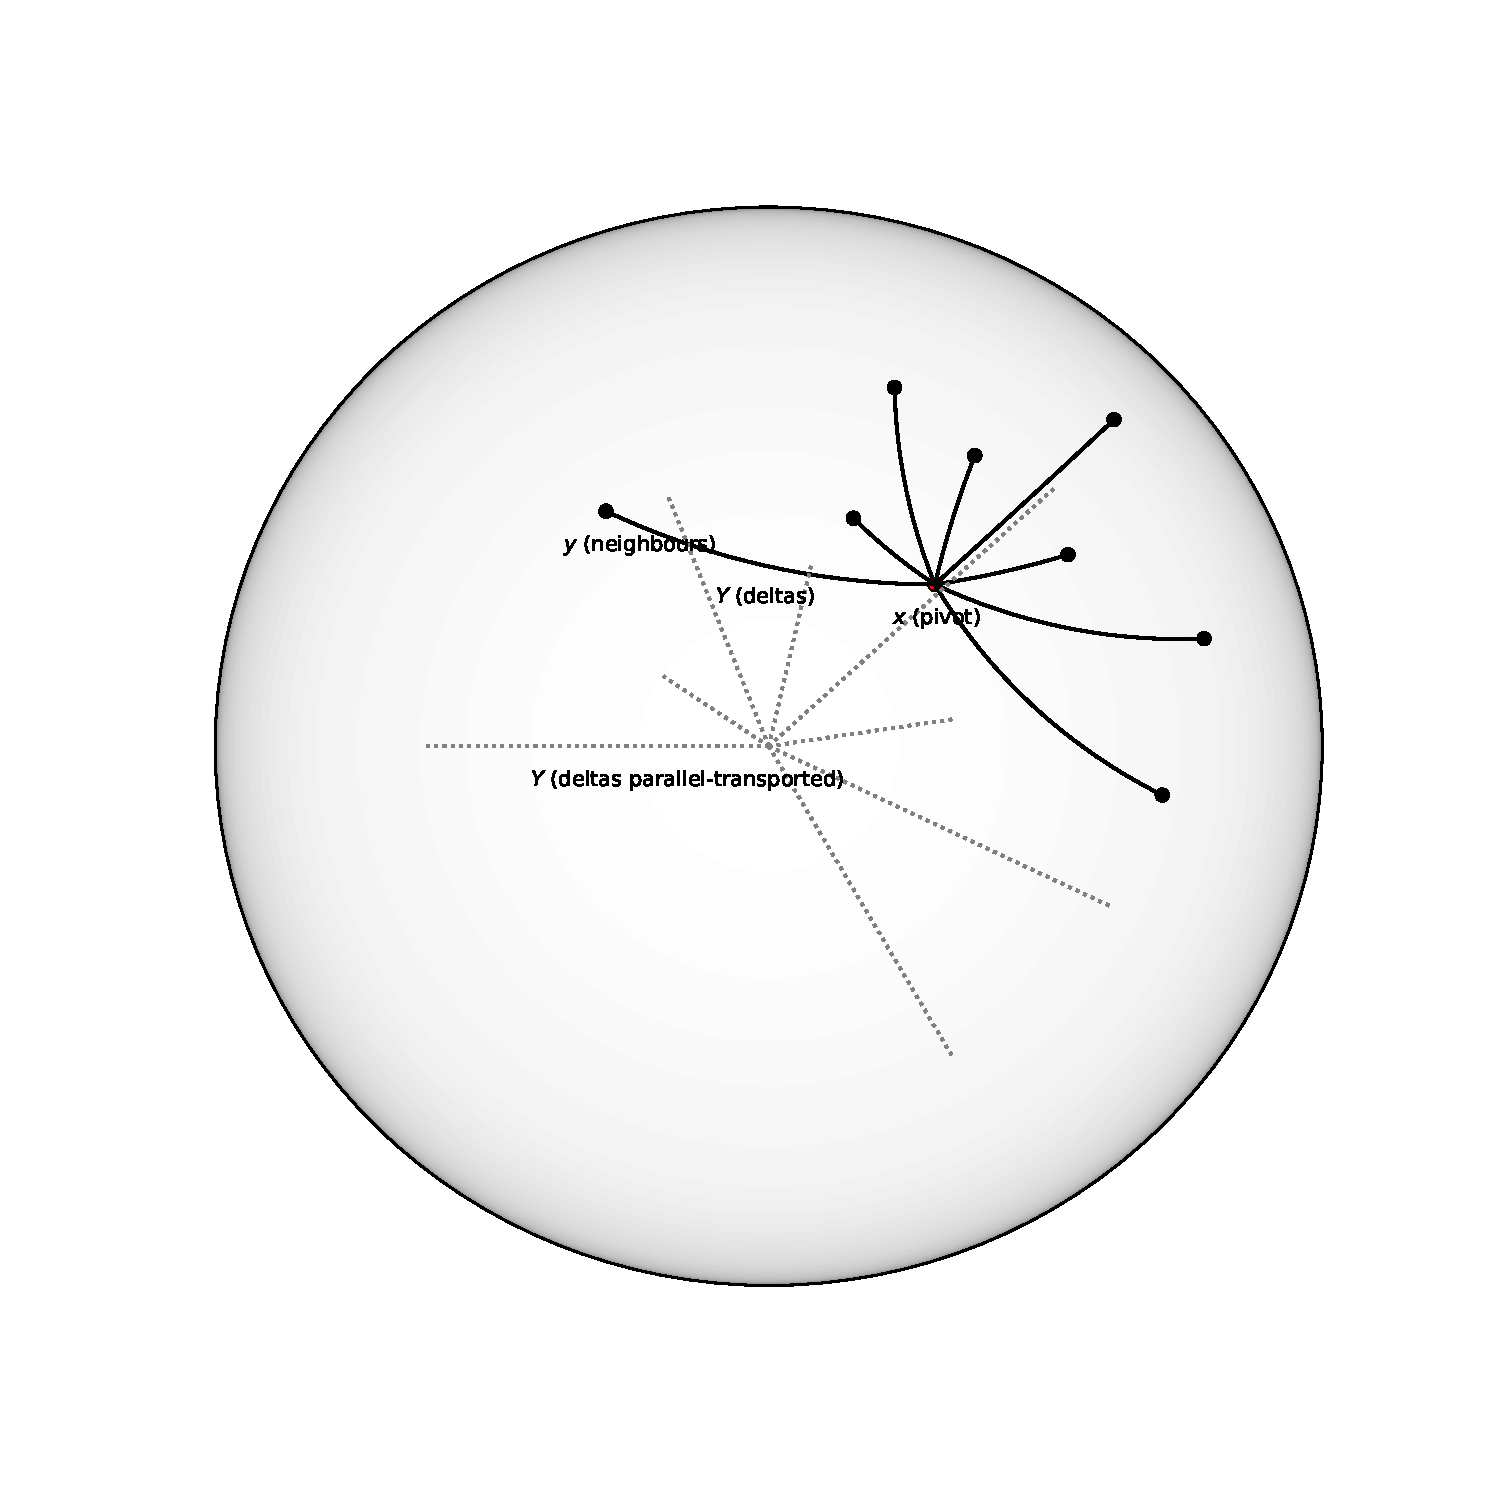
\includegraphics[width=.9\textwidth]{art/neighbours.pdf}
\caption{Relative directions to neighbour embeddings. To an embedding \( y \)
there corresponds a tangent vector \( Y = \log_x y \), visualized here as a
geodesic line segment in Poincar\'e ball.}
\end{figure}

\section{Hyperbolic EdgeConv} \label{sec:hedgeconv}

\citet{edgeconv} propose a convolutional layer that operates directly on
pointclouds (producing a ``cloud of embeddings'' after each step, similar to
how we produce a regular \( 2 \)D \emph{array} of embeddings in the section
above). This layer dynamically constructs a \( k \)-nearest neighbours graph
from the input pointcloud, and then transforms each point by aggregating it
with adjacent nodes. Specifically, for each neighbour of a node under
consideration, a message is constructed using an MLP that ``eats'' a point and its
location relative to the node. A pooling is then used to aggregate the messages
and produce the output point.

Replacing the subtraction with logarithmic map in message formation, and using
manifold distances when constructing \( k \)-NN graph, we can generalize the
operation to hyperbolic embeddings. A number of concerns remain: the original
model uses Batch Normalization and rectifying non-linearities. Search for
meaningful non-linearities for hyperbolic neural networks remains an open
problem. Batch Normalization is straightforwardly generalized, but only
partially: mean and variance make perfect sense in a general metric space
setting, but \emph{co}variances inherently rely on the product-structure of
vector space-valued random variables.

We note that our convolutions for arrays of hyperbolic points from the previous
section are an instance of such EdgeConv, if an image is treated as a
regular grid-like graph. In particular, in our implementation of EdgeConv we
allow image inputs by deleting \textrm{KNNEdges} layer that dynamically
constructs the \( k \)-NN graph from the input.

\begin{figure}[H]\center
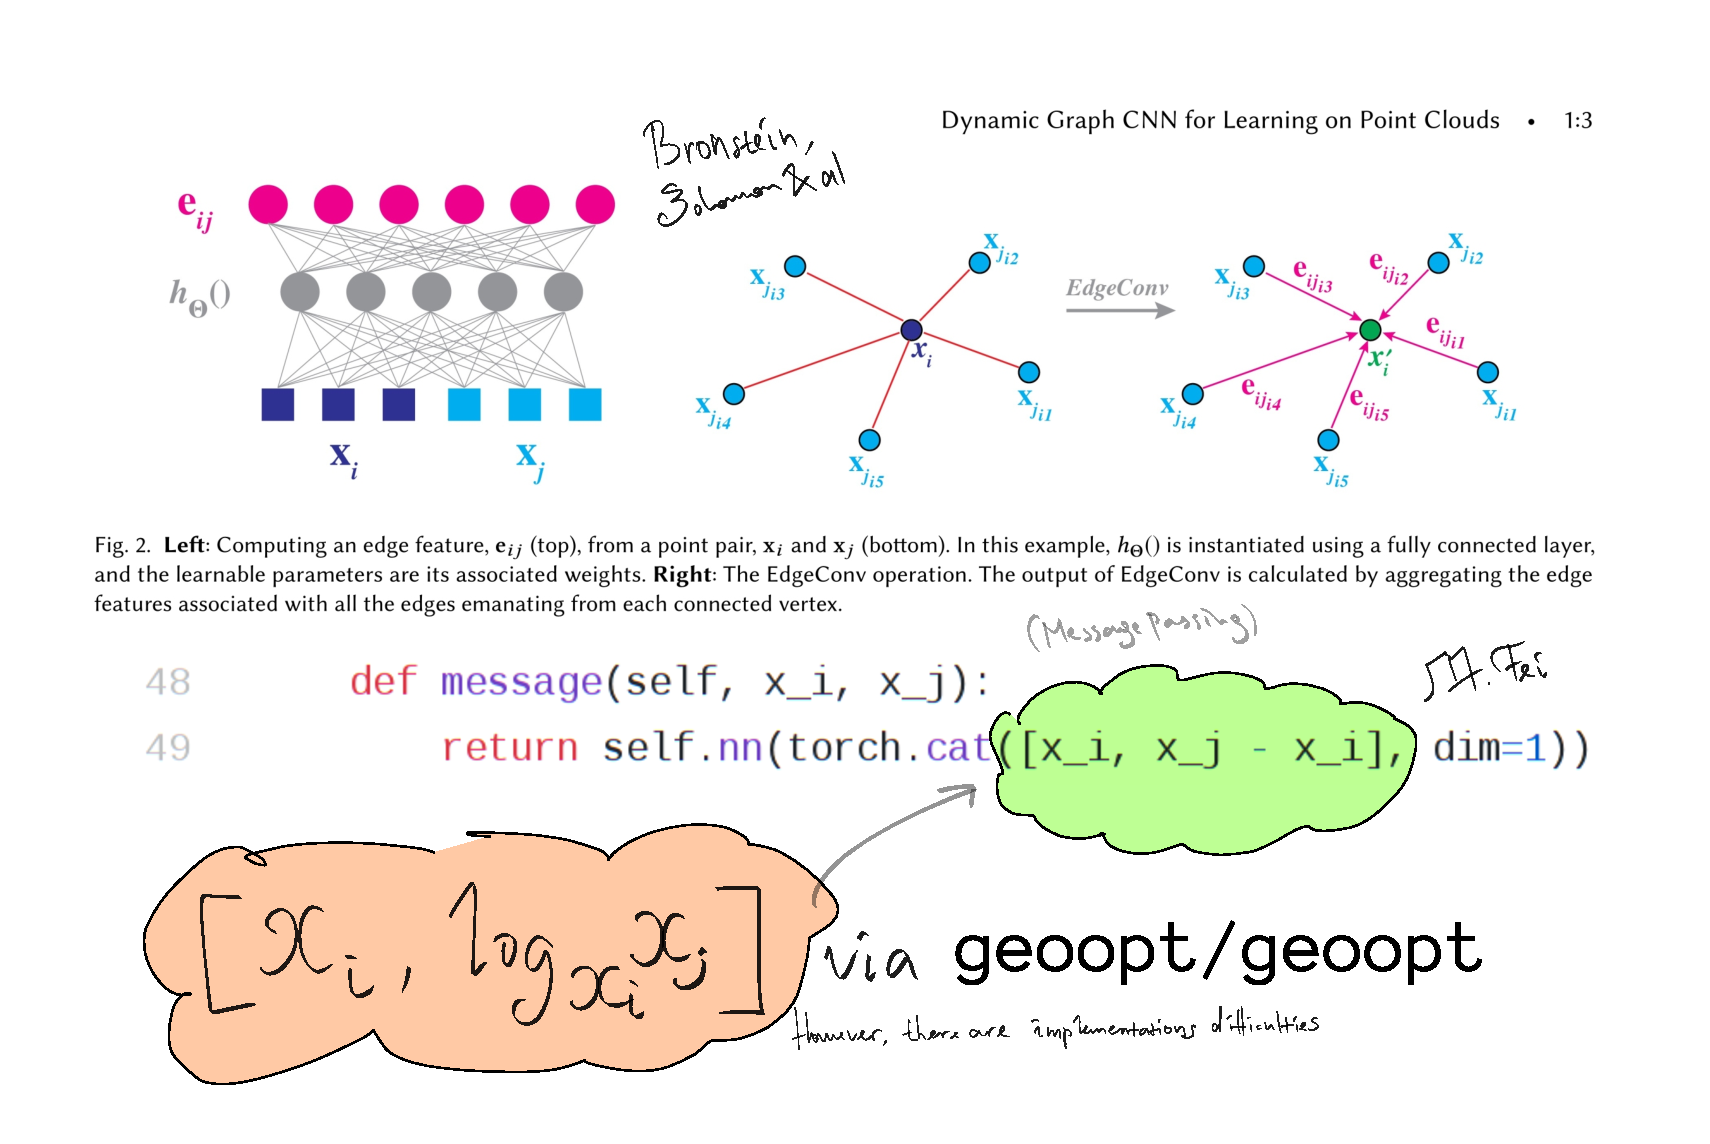
\includegraphics[width=.9\textwidth]{art/hyperbolic-edgeconv.pdf}
\caption{
    Visualization of EdgeConv from~\citet{edgeconv} and the change
        required to EdgeConv implementation of~\citet{pytorchGeometric}
}
\end{figure}

\section{Evaluation and results} \label{sec:results}

Just as the model in \autoref{sec:hconv}, our model (\autoref{sec:hconv-new})
proved to heavily suffer from overfitting and fail to learn under reasonable
regularization.  Our
naive hyperbolic edge convolution (\autoref{sec:hedgeconv}) slightly
under-performs compared to
baselines, but requires much fewer parameters. However, that comes at the cost of
longer iterations. In~\autoref{fig:hedgeconvAccCurve} one can see
the accuracy of our model evaluated on classification of Modelnet40
dataset and in~\autoref{fig:edgeconvComparison} the comparison
against baselines.

\begin{table}[h!]
\centering
\begin{tabular}{|c c c c c c|} 
 \hline
 Model & \(\sharp\) parameters & \( \sharp \) epochs & PCD size & Accuracy & Class-balanced
 \\ [0.5ex] 
 \hline\hline
 EdgeConv & \( 1 \)M & ?  & \(1024\) & \(.92\) & \(.902\)  \\ 
 3DShapeNets & \( 5 \)M & \( ? \)  & \( ? \) & \(.847\) & \(.773\)  \\ 
 OURS & \( 85 \)K & 10 & 768 & \(.785\)  & \( .712 \) \\ [1ex] 
 \hline
\end{tabular}
\caption{Comparison of results on Modelnet40 classification.  Our main
reference is the original~\citet{edgeconv} as is not too far from SOTA and we
haven't yet beaten it as a baseline anyway. \citet{edgeconv} also note
that ``with fewer than \( 512 \) points [in the pointcloud subsample]
the performance degenerates dramatically'', however we were only able
to evaluate the model with \( 512 \)--\( 768 \) points -- our
experimental abilities are limited by what free Google Colaboratory has
to offer}
\label{fig:edgeconvComparison}
\end{table}

\begin{figure}[h]\center
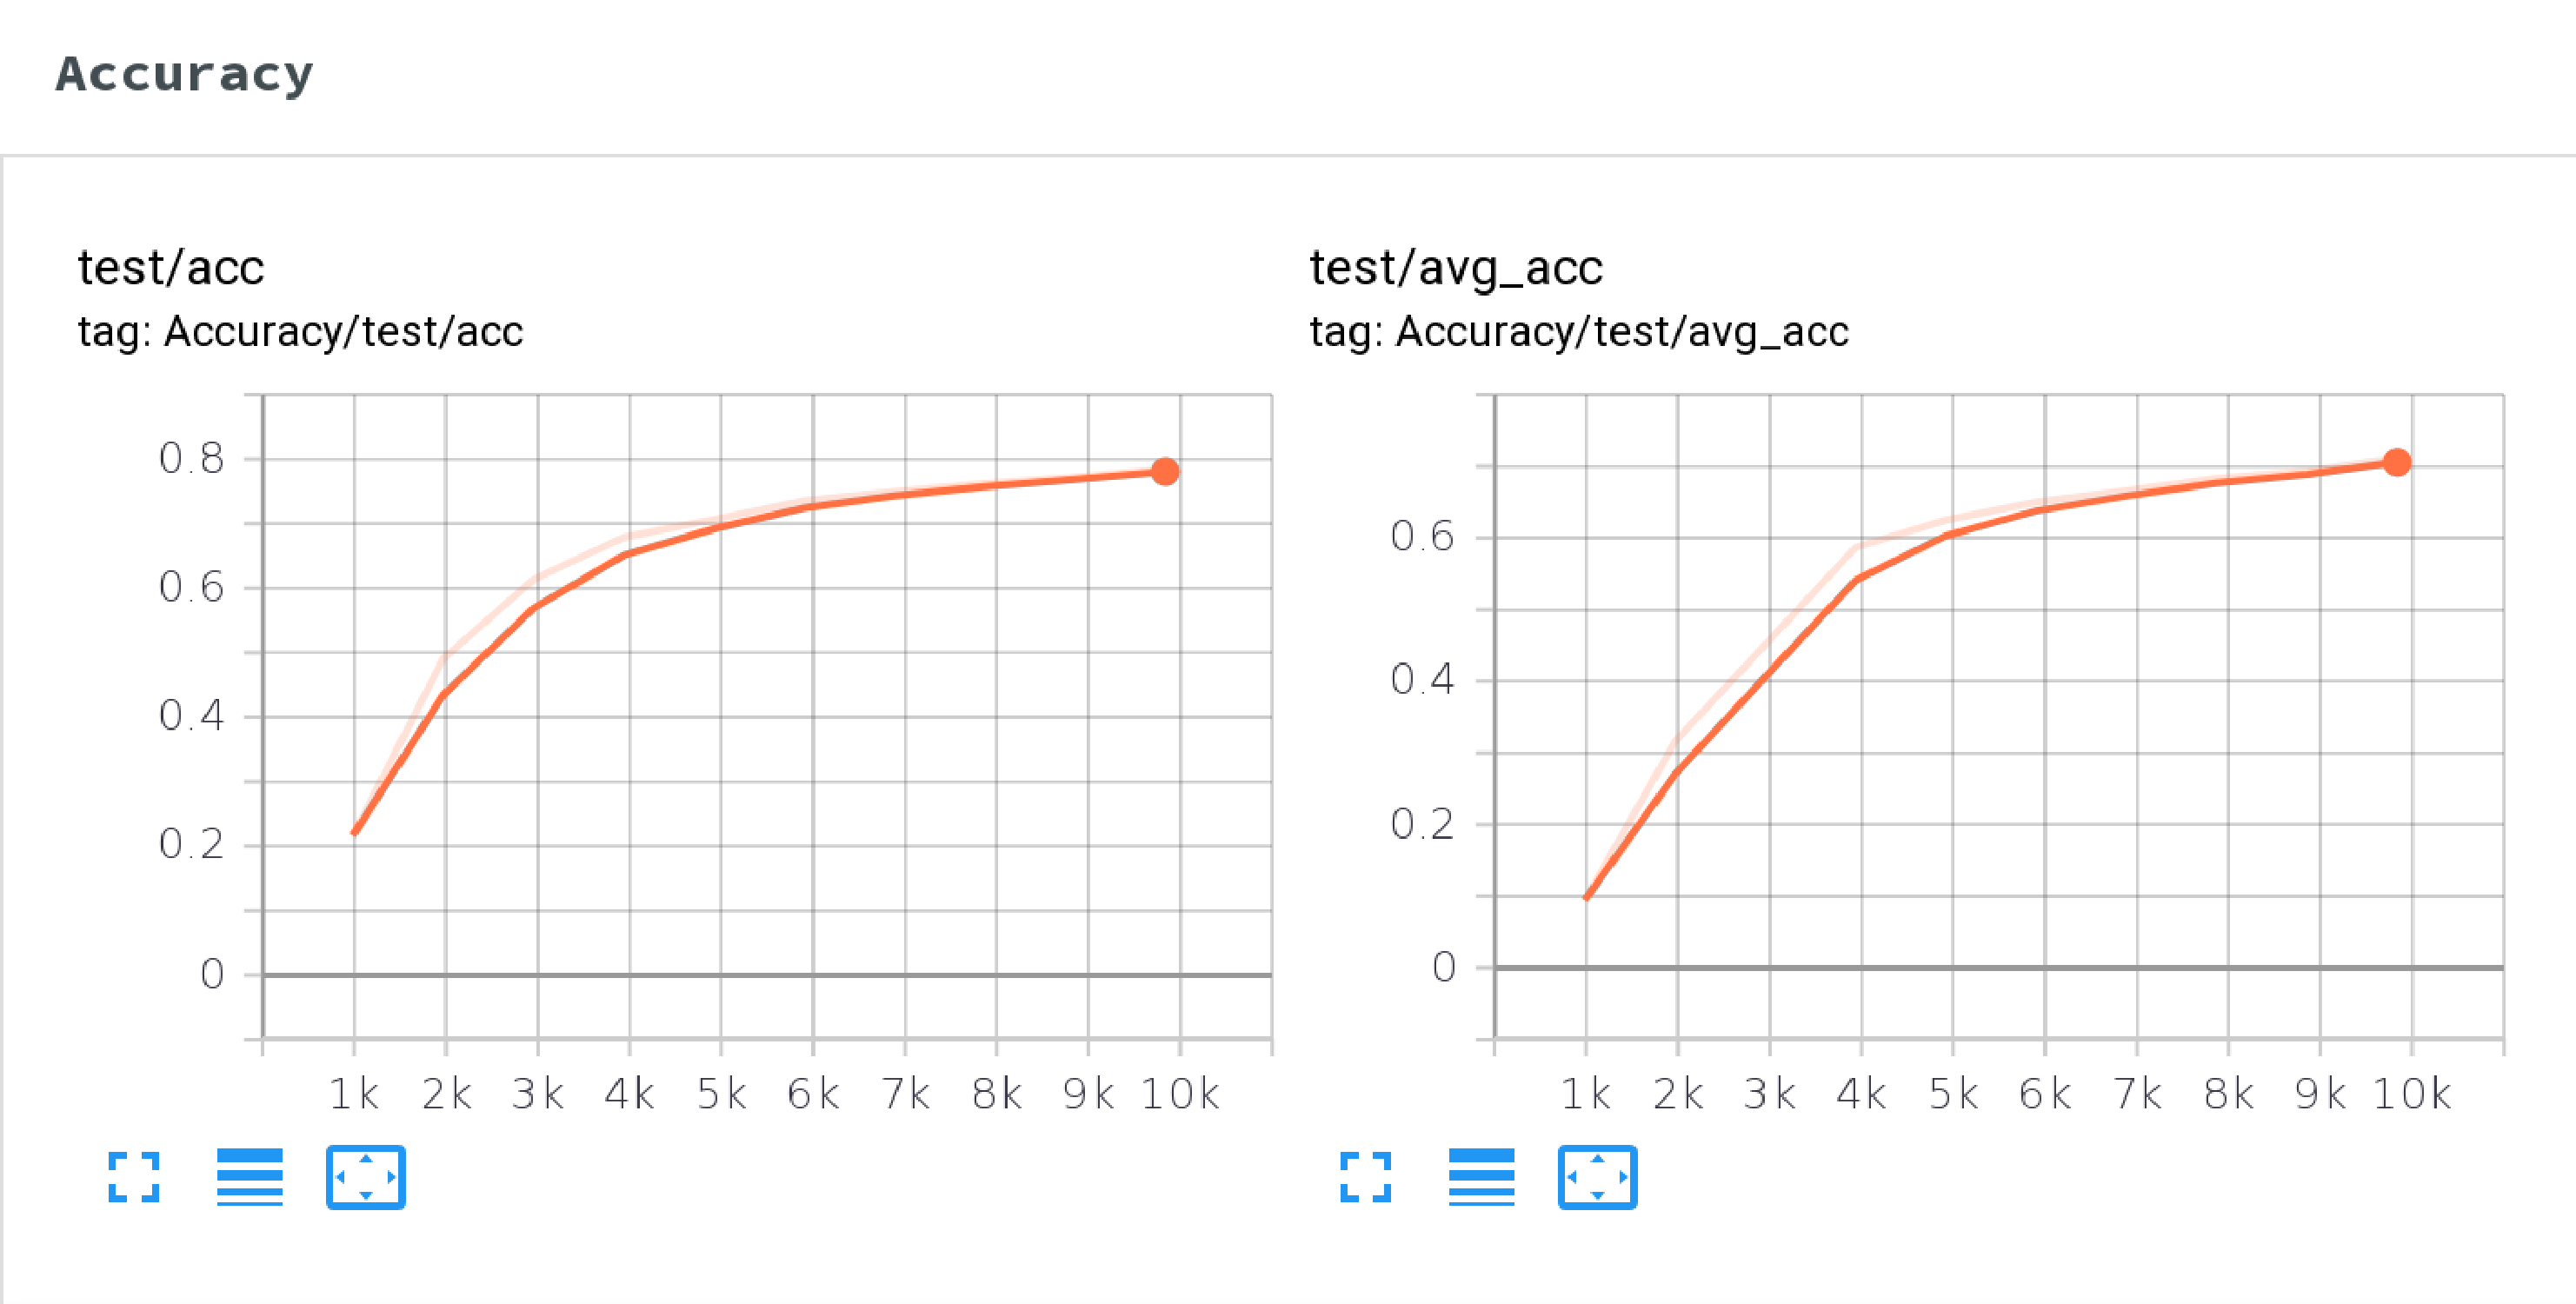
\includegraphics[width=.9\textwidth]{art/hedgeconv-tensorboard.pdf}
\caption{Accuracy and class-balanced accuracy of hyperbolic EdgeConv with 85K
parameters on Modelnet40 classification}
\label{fig:hedgeconvAccCurve}
\end{figure}

\section{Discussion} \label{sec:discussion}

There are several conceptual inconsistencies with considered models.  First
of all, in both cases, the ``convolution'' happens along the spatial dimensions
(over window pixels in an image, and over graph edges in EdgeConv). The image
case is especially good at illuminating the inconsistency: our input is a
signal on Euclidean plane, and we're trying to construct an operation invariant
with respect to... what group exactly? While this is not what we did, think
what sense does M\"obius transformation of a photograph make? It's a type
mismatch.
\citet{s2cnn} carefully reformulate a problem at hand so that the input to the
model is a signal on a sphere, and apply a classic convolution equivariant with
respect to the group of rotations. Similarly, for our ``convolutions of
hyperbolic arrays'' or ``hyperbolic edge convolutions'', we shall first find an
interpretation of our input as a signal on certain space and then describe an
operation invariant (or equivariant) with respect to appropriate
transformations. Such operation should be interpretable as aggregation in EdgeConv,
and also follow the intuition of the ``continuous trees'' metaphor as
in~\autoref{sec:hconv}. In our current models we involuntarily interpret
hyperbolic points within the sliding window as a trivial hyperbolic signal (sum
of point-mass measures). By taking the logarithmic map from one of the points in the
window, we make our ``convolution'' invariant with respect to translations of
hyperbolic space. However we might desire equivariance with respect to
all unit ball-preserving M\"obius transformations (isometries of Poincar\'e disk)
and we could employ the technique similar to~\cite{s2cnn} and integrate
over the entire group of isometries. We cannot hope to implement that efficiently
without the tricks of Harmonic analysis. \citet{stollharmonic} works out the
Harmonic analysis on real Hyperbolic space, including the spherical harmonics.
We should also note that our singular (combination of delta measures)
signal might turn out not to be the most convenient to work with in terms of
complexity of computations, nor the most representative one. In other words, we
must reconsider the way we construct and represent a signal on a Hyperbolic
space. Finally, the problem of coming up with meaningful nonlinearities
for general manifolds and particularly Hyperbolic spaces remains open.

\section{Conclusion}

In~\autoref{sec:statement} we have discussed naive convolutional layers for
hyperbolic representations and found these implementations to be insufficient
to achieve the desired performance. In~\autoref{sec:discussion} discussed why
these models may have failed and concluded that our experiments don't allow to
confidently discard the idea and that more ingenious implementations are
needed.  There, we also described the principles on which to build refined
models.  In~\nameref{chap:manifolds} we made an attempt to describe the
language and the general framework in which we would like to see geometric
methods to be treated.  In~\nameref{sec:geoopt} we discussed current challenges
for optimization on manifolds for deep learning.
